\chapter{Spatial and Entity-Based Neural Architectures}
\label{chap:architectures}

The neural network is the function approximator that PPO optimizes. Its capacity and inductive bias bound what the agent can ultimately represent. Seven architectures are presented in this chapter, each adding one or two contributions on top of the previous one. The progression is therefore incremental by construction. Rather than presenting these architectures chronologically, the chapter organizes the architectural requirements of an RTS network into three spatial and relational reasoning axes; temporal and curriculum aspects are addressed in Chapter~\ref{chap:training-system}. Each contribution naturally targets one specific axis. Section~\ref{sec:axes} introduces these three axes and the actor-critic skeleton common to all seven networks. Sections~\ref{sec:axis-local} to~\ref{sec:axis-global} present the architectures that progressively address each axis. Section~\ref{sec:uecd} synthesizes the contributions into the final \code{UECD} architecture. Section~\ref{sec:arch-summary} provides a recap table of all seven designs, whose contributions are quantified empirically in the architecture ablation of Chapter~\ref{chap:results}.

\section{Common Skeleton and Reasoning Axes}
\label{sec:axes}

\subsection{Actor-Critic Skeleton}
\label{subsec:skeleton}

All seven architectures follow the shared-encoder actor-critic pattern recalled in Chapter~\ref{chap:rl_basis}. A single encoder $f_{\boldsymbol{\theta}}$ first compresses the observation tensor (Section~\ref{sec:obs-encoding}) to a bottleneck representation of shape $(B, C', H', W')$, where $C'$ is an architecture-dependent channel count, $(H', W')$ the compressed spatial resolution and $B$ the batch size (the $N$ parallel environments of Chapter~\ref{chap:python_bridge} during rollout, or the minibatch size during the PPO update). A decoder then upsamples this representation back to full resolution $(B, C'', H, W)$ before it is consumed by the two heads. Sharing this encoder-decoder backbone between the actor and the critic, rather than training two independent networks, roughly halves the parameter count for the same representational capacity, since both heads need the same spatial features (unit positions, threat regions, resource distribution). The actor head outputs per-cell logits of shape $(B, H, W, 78)$, factored as in Section~\ref{sec:action-space} and masked to $-10^8$ before sampling. The critic head outputs a scalar value estimate $\hat{V}(s)$.

\subsection{Three Reasoning Axes}
\label{subsec:axes}

Strategic play in MicroRTS requires three qualitatively different forms of reasoning:

\paragraph*{1. Local spatial reasoning.} Most tactical decisions are settled within a unit's immediate neighborhood: which adjacent cell to step into, which neighbor to attack, where to deposit a carried resource. A Worker-vs-Worker engagement on a contested resource patch is decided entirely by the local configuration of the two units and the adjacent terrain. Convolutional layers are the canonical inductive bias for this regime~\cite{stanescuEvaluatingRealtimeStrategy2016}: their translation equivariance encodes the prior that such an engagement looks the same whether it occurs near the home base or at the opposite corner of the map, and weight sharing extracts the same tactical patterns from any position with a fraction of the parameters of a fully connected alternative.

\paragraph*{2. Long-range relational reasoning.} Units act as a coordinated group, and the relationships that matter are \emph{entity-to-entity} rather than cell-to-cell. A Heavy advancing in front of friendly Ranged units must absorb incoming damage while the Ranged behind focus their fire on the same enemy to bring it down within a single tick; a Worker rush detected at the opponent base should trigger a defensive recall regardless of how far the defenders stand. These dependencies are sparse, since only the $n_t$ active units participate rather than $H{\times}W$ cells, and irregular, since any pair of units may interact at any spatial separation. A purely convolutional backbone captures them only indirectly, through stacked receptive fields that must grow until they happen to overlap the relevant units. Self-attention over unit tokens fits this structure directly, computing pairwise interactions at any distance in a single layer.

\paragraph*{3. Global spatial reasoning.} A third class of decisions hinges on region-to-region trade-offs not localized to any specific entity: committing to a frontal push vs answering pressure on the home base, or shifting production between two barracks on opposite sides of the map. Standard CNNs reach such a global view only by stacking enough downsampling layers for the receptive field to span the map, which mixes long-range information with the strong locality bias of convolutions and dilutes the signal. Spatial self-attention applied at the bottleneck provides this view directly: every spatial token attends to every other in a single layer, at a cost quadratic in the reduced number of tokens rather than the full grid.

\medskip

Existing convolutional architectures for MicroRTS, including GridNet~\cite{huangGym$m$RTSAffordableFull2021} and the DoubleCone backbone of RAISocketAI~\cite{goodfriendCompetitionWinningDeep2024}, primarily address the local axis and capture long-range dependencies only indirectly through stacked convolutions and downsampling. The final architecture of this thesis (Section~\ref{sec:uecd}) covers the three axes explicitly through three complementary mechanisms: a CNN backbone for local reasoning, a Transformer encoder over unit tokens for relational reasoning, and a self-attention layer over the bottleneck grid for global reasoning. This three-way design mirrors AlphaStar's entity-spatial pair (Section~\ref{sec:alphastar}), adapted here to MicroRTS scale.

\section{Axis 1: Local Spatial Reasoning}
\label{sec:axis-local}

Three architectures (\code{GridNet}, \code{IMPALA-CNN}, \code{U-Net}) progressively refine the convolutional backbone responsible for the local axis. Convolutional Block Attention Module (CBAM), a more expressive attention module, is introduced here and later folded onto \code{U-Net-Entity}.

\paragraph{GridNet.}
\code{GridNet}~\cite{hanGridWiseControlMultiAgent2019}, with per-cell action prediction motivated in Section~\ref{sec:microRTS_sota}, serves as the baseline, following the implementation of~\cite{huangGym$m$RTSAffordableFull2021}. Its encoder applies four convolutional blocks ($3{\times}3$ convolution, ReLU (Rectified Linear Unit) activation function, stride-2 max-pooling), expanding channels as $C \to 32 \to 64 \to 128 \to 256$ and collapsing the spatial resolution to a $1{\times}1$ bottleneck. The actor mirrors this path with four transposed convolutions; the critic flattens the $256$-dimensional bottleneck through a two-layer MLP. Two limitations follow. First, the extreme bottleneck discards spatial detail that the per-cell decoder must then reconstruct from a single $256$-dimensional vector. Second, the flatten in the critic ties the network to a fixed map size of $16{\times}16$.

\paragraph{IMPALA-CNN.}
\code{IMPALA-CNN} replaces \code{GridNet}'s plain convolutions with the residual encoder of the Importance-Weighted Actor-Learner Architecture (IMPALA)~\cite{espeholtIMPALAScalableDistributed2018}: three stages of \{Conv $\to$ MaxPool $\to$ 2${\times}$ResBlock\} producing 32, 64, and 128 channels and compressing the spatial resolution to $H/8 \times W/8$. Each ResBlock follows a pre-activation scheme (ReLU $\to$ Conv $\to$ ReLU $\to$ Conv $+$ skip). These residual blocks enable the deeper backbones of subsequent architectures without unstable gradient flow. The decoder mirrors the encoder with transposed convolutions, and the critic replaces \code{GridNet}'s fixed flatten with adaptive average pooling. From this architecture onward, the network is decoupled from the map resolution and can be used in the padded multi-map training environment of Section~\ref{subsec:padding}.

\paragraph{U-Net.}
U-shaped Neural Network (\code{U-Net}) introduces two changes to the IMPALA-CNN backbone. First, \code{U-Net} skip connections~\cite{ronnebergerUNetConvolutionalNetworks2015} route encoder features at matching resolutions directly into the decoder before each upsampling stage, addressing the spatial detail loss observed at the \code{GridNet} and \code{IMPALA-CNN} bottlenecks; attention gates on such skip connections have also been studied~\cite{oktayAttentionUNetLearning2018}. The encoder uses three stages with two stride-2 convolutions instead of max-pooling, reaching a spatial resolution of $H/4 \times W/4$. Second, every residual block is gated by SE channel attention~\cite{huSqueezeandExcitationNetworks2018}, the same mechanism used in RAISocketAI's DoubleCone backbone (Section~\ref{sec:microRTS_sota}): global average pooling and a bottleneck MLP produce a per-channel importance vector that rescales feature maps to emphasize channels relevant to the current situation.

\paragraph{CBAM attention.}
CBAM~\cite{wooCBAMConvolutionalBlock2018} replaces SE in every residual block, extending it with an explicit spatial attention stage (Figure~\ref{fig:cbam-resblock}). The feature map is pooled along the channel axis (average and max), the two saliency maps are concatenated, and a $7{\times}7$ convolution followed by a sigmoid produces a per-position weight in $[0,1]^{H{\times}W}$. The channel gate inherited from SE is applied first, emphasizing situationally relevant feature maps (e.g., Ranged-unit and HP channels during combat); the spatial gate follows, emphasizing critical map regions (contested frontlines, exposed worker positions, choke points). A residual connection then adds the block input back before the final ReLU. The parameter overhead over SE is negligible (${\approx}100$ weights per block).

\begin{figure}[!htb]
    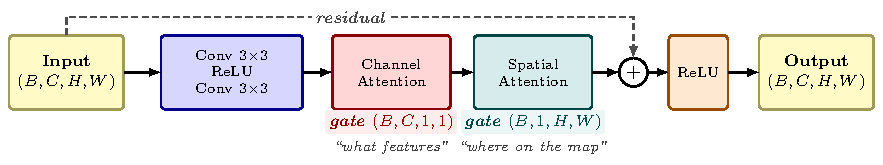
\includegraphics[width=\linewidth]{chapters/08_architectures/figures/cbam_resblock_simplified.pdf}
    \caption[CBAM-ResBlock (simplified view)]{CBAM-ResBlock (simplified view). Channel attention selects \emph{what features} matter; spatial attention selects \emph{where on the map} to look. Residual shown in gray dashed.}
    \label{fig:cbam-resblock}
\end{figure}

\vspace{-0.5cm}

\section{Axis 2: Long-Range Relational Reasoning}
\label{sec:axis-relational}

Although stacked convolutions can in principle bridge long spatial distances, the resulting cell-level features blur identifiable units into pooled channel statistics: two units twenty grid steps apart interact only through several rounds of downsampling, and the output represents not the two specific units but the activity of their respective regions. The relational axis preserves unit identity by maintaining one explicit token per controllable unit and processing the resulting set with a Transformer encoder~\cite{vaswaniAttentionAllYou2017, zwingenbergerTransformersPoliciesVariable2023}, following AlphaStar's entity-spatial pair (Section~\ref{sec:alphastar}). 

\paragraph{Token construction.}
For each unit on the grid (friendly or enemy), a token is built by concatenating three complementary sources: raw observation features carry unit-specific semantics (type, HP, carried resource, current action) that the CNN may have abstracted away; the CNN features encode spatial context (nearby allies, terrain, threats); and the normalized grid coordinates $(\mathrm{row}, \mathrm{col})$ make position recoverable, which the permutation-invariant attention would otherwise discard. A linear projection maps each token to $d_{\mathrm{model}} = 128$, then a two-layer, four-head Transformer encoder processes the resulting $(B, n_t, 128)$ tensor. Since strategic decisions depend equally on intra-player coordination (which Worker should harvest where) and inter-player relations (which enemy Ranged threatens which Light), every unit attends to every other regardless of ownership, with no relational mask; a padding mask only hides unused slots in the fixed-size tensor. The two layers and four heads provide enough relational depth to capture multi-hop interactions.

The enriched representations are projected back to spatial channels and scattered into the convolutional stream by additive insertion at each unit's downsampled grid position. The per-step cost remains manageable at MicroRTS unit counts ($n_t$ is bounded by the unit cap, keeping $\mathcal{O}(n_t^2)$ small) and is acceptable relative to the representational gain (quantified in Chapter~\ref{chap:results}). It does, however, noticeably reduce throughput, as shown in Table~\ref{tab:arch-summary}.

\paragraph{IMPALA-CNN-Entity.}

\code{IMPALA-CNN-Entity} is the first integration. A lightweight full-resolution CNN (two $3{\times}3$ convolutions, 64 channels) runs in parallel with the \code{IMPALA-CNN} encoder to provide the per-cell features used in token construction, since the \code{IMPALA-CNN} bottleneck is too coarse. The enriched tokens are projected and scattered back at the \code{IMPALA-CNN} bottleneck only. Two limitations follow: the parallel CNN performs redundant feature extraction that the main encoder also does at lower resolution, increasing parameters without sharing computation; and the single bottleneck-scale scatter dilutes the entity information by the time the decoder reaches full resolution.

\paragraph{U-Net-Entity.}

\code{U-Net-Entity} combines the Entity Transformer with the \code{U-Net} backbone of Section~\ref{sec:axis-local}, removing both inefficiencies of the previous design. The parallel CNN is replaced by \code{U-Net}'s full-resolution skip connection \emph{skip1}, which already encodes high-quality features. Enriched representations are then scattered back at two scales rather than one: into the bottleneck ($H/4 \times W/4$) for global strategic reasoning (army composition, resource allocation), and into the mid-resolution skip connection \emph{skip2} ($H/2 \times W/2$) for spatially precise per-unit influence (positioning, target selection). When multiple units fall in the same target cell after downsampling (more frequent at the bottleneck than at \emph{skip2}), their projected embeddings are summed via PyTorch's \code{index\_add\_}, a permutation-invariant aggregation that preserves all per-unit contributions without averaging or learned pooling. Figure~\ref{fig:entity-transformer} summarizes the mechanism end-to-end with this backbone.

\begin{figure}[!htb]
      \centering
      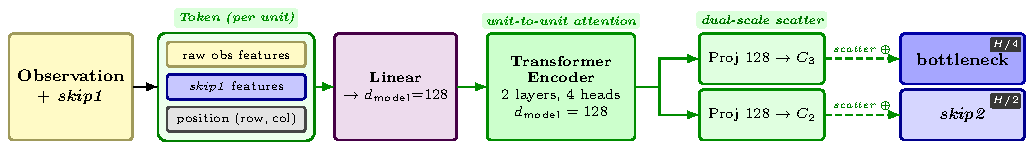
\includegraphics[width=\linewidth]{chapters/08_architectures/figures/entity_transformer_simplified.pdf}
      \caption[Entity Transformer mechanism (simplified view)]{Entity Transformer mechanism (simplified view) with the \code{U-Net} backbone.}
      \label{fig:entity-transformer}
\end{figure}

\vspace*{-0.5cm}

\paragraph{U-Net-Entity-CBAM.}
Folding the CBAM gate of Section~\ref{sec:axis-local} onto \code{U-Net-Entity} yields \code{U-Net-Entity-CBAM}, the sixth architecture. It adds spatial attention on top of the relational backbone at negligible parameter cost, isolating the contribution of the spatial gate in the ablation of Chapter~\ref{chap:results}.

\section{Axis 3: Global Spatial Reasoning}
\label{sec:axis-global}

Decisions such as committing to a frontal push while pressure mounts on the home base require relating features at opposite ends of the map in a single forward pass. Convolutions are local operators. The theoretical receptive field of a stride-2 $3{\times}3$ convolutional stack grows only as $\mathcal{O}(2^d)$ with depth $d$, and the effective receptive field is known to be substantially smaller~\cite{luoUnderstandingEffectiveReceptive2017}; even on $16{\times}16$ maps, a unit at one edge cannot reliably attend to the opposite edge through convolutions alone. Two complementary mechanisms address this limitation.

\paragraph{Bottleneck self-attention.}
A four-head spatial self-attention layer is inserted after the bottleneck residual blocks. Each spatial position at the bottleneck is treated as a token of dimension $C_3 = 4 C_1$, and standard multi-head self-attention~\cite{vaswaniAttentionAllYou2017} is applied across all tokens, allowing every position to attend to every other regardless of distance. The placement at the deepest stage keeps the cost small: at $H/4 \times W/4$ the grid holds $16\times$ fewer tokens than the full-resolution map, so the $\mathcal{O}(N^2)$ self-attention is $16^2 = 256\times$ cheaper than at full resolution.

\paragraph{Pyramidal depth profile.}

Earlier architectures use a uniform two residual blocks per \code{U-Net} stage. This is replaced by the configuration $(2, 3, 4, 3, 2)$, peaking at four blocks at the bottleneck. Capacity is concentrated there for two reasons. First, bottleneck features synthesize information from the full map and serve two roles: feeding the global self-attention module and receiving the Entity Transformer's scattered output. Depth there therefore has the largest strategic effect. Second, the bottleneck's small spatial resolution makes computation cheapest.

\vspace{-0.7em}

\section{UECD: Final Architecture}
\label{sec:uecd}

\vspace{-0.25em}

The final architecture, \code{UECD} (U-Net-Entity-CBAM-Deep), combines the contributions of the three previous sections. Figure~\ref{fig:arch-cbam-deep} shows the simplified structure, with ${\approx}4.7$\,\text{M} parameters at the default base width $C_1 = 48$ and the $73$-channel extended observation encoding (Section~\ref{sec:obs-encoding}). The fully annotated architecture with all channel widths and tensor dimensions is presented in Appendix~\ref{app:arch-diagrams}.
  
\begin{figure}[!htb]
    \centering
    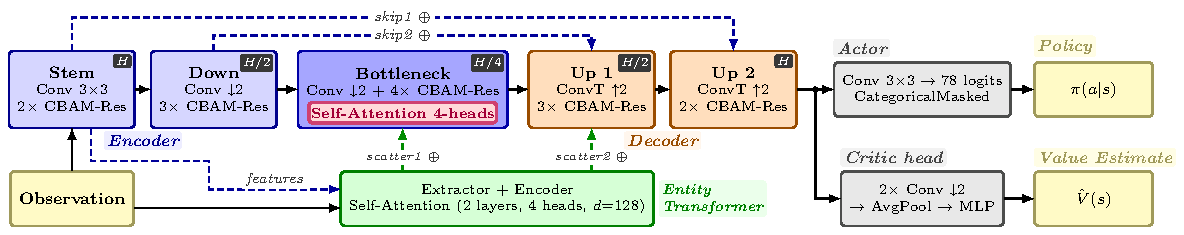
\includegraphics[width=\textwidth]{chapters/08_architectures/figures/arch_uecd_simplified.pdf}
    \caption[\code{UECD} architecture (simplified view)]{\code{UECD} architecture (${\approx}4.7$\,\text{M} parameters at $C_1{=}48$). Top: CBAM-gated \code{U-Net} backbone (blue encoder, orange decoder) with pyramidal depth profile $(2, 3, 4, 3, 2)$ and bottleneck self-attention (red). Bottom: Entity Transformer (green) extracts per-unit features and scatters back into the bottleneck and \emph{skip2} (green dashed). \code{U-Net} skips between encoder and decoder (blue dashed).}
    \label{fig:arch-cbam-deep}
\end{figure}

\vspace{-0.5em}

The four modules of \code{UECD} map onto the three reasoning axes as follows. The CBAM-gated \code{U-Net} backbone realizes the local spatial axis (Section~\ref{sec:axis-local}). The Entity Transformer with dual-scale scatter into the bottleneck and \emph{skip2} realizes the relational axis (Section~\ref{sec:axis-relational}). The bottleneck self-attention layer, together with the pyramidal depth profile $(2, 3, 4, 3, 2)$ that concentrates capacity there, realizes the global spatial axis (Section~\ref{sec:axis-global}). The actor and critic heads read from the decoder's full-resolution output: the actor applies a single $3{\times}3$ convolution mapping $C_1$ channels to the 78 per-cell action logits (masked and sampled as in Section~\ref{sec:action-space}), while the critic applies two stride-2 $3{\times}3$ convolutions, an adaptive average pool to $1{\times}1$, and a two-layer MLP, producing $\hat{V}(s)$.

\vspace{-0.7em}

\section{Architecture Summary}
\label{sec:arch-summary}

\vspace{-0.25em}

Table~\ref{tab:arch-summary} recaps the seven architectures, whose empirical contributions are quantified in Section~\ref{sec:arch-sweep}.

\begin{table}[!ht]
\centering
\caption[Overview of the seven architectures]{Overview of the seven architectures.}
\label{tab:arch-summary}
\small
\renewcommand{\arraystretch}{0.9}
\begin{tabularx}{\textwidth}{@{}l r r c X@{}}
\toprule
\textbf{Architecture} & \textbf{Params} & \textbf{SPS\textsuperscript{\dag}} &
\textbf{Axes\textsuperscript{\ddag}} & \textbf{Key addition} \\
\midrule
GridNet                & $838$\,\text{k}    & $2\,688$ & S       & Baseline encoder-decoder \\
IMPALA-CNN                 & $1.02$\,\text{M}   & $2\,416$ & S       & + Residual blocks, adaptive critic pool \\
U-Net                   & $2.59$\,\text{M}   & $2\,121$ & S       & + U-Net skips, SE attention \\
\midrule
IMPALA-CNN-Entity          & $1.37$\,\text{M}   & $1\,903$ & S\,/\,R    & + Entity Transformer \\
U-Net-Entity            & $2.90$\,\text{M}   & $1\,518$ & S\,/\,R    & + Entity scatter integrated with U-Net (dual-scale)
\\
U-Net-Entity-CBAM       & $2.90$\,\text{M}   & $1\,289$ & S\,/\,R    & + Spatial attention (CBAM) \\
\midrule
\textbf{U-Net-Entity-CBAM-Deep}          & $4.72$\,\text{M}   & $1\,176$ & S\,/\,R\,/\,G & + Pyramidal depth profile, self-attention \\
\bottomrule
\multicolumn{5}{@{}l}{\textsuperscript{\dag}\scriptsize Steps per second, measured on \emph{basesWorkers16x16A}
with $24$ parallel environments.}\\[-4pt]
\multicolumn{5}{@{}l}{\textsuperscript{\ddag}\scriptsize Axes covered: \textbf{S} $\equiv$ local
\textbf{S}patial, \textbf{R} $\equiv$ \textbf{R}elational, \textbf{G} $\equiv$ \textbf{G}lobal spatial.}
\end{tabularx}
\end{table}